%\documentclass{report}
%\documentclass[11pt,twoside,a4paper]{report}
\documentclass[11pt,journal,compsoc]{report}[1]
\usepackage[letterpaper, margin=0.75in]{geometry}
\usepackage{lipsum}
\usepackage{epstopdf}
\usepackage{amsthm}
\PassOptionsToPackage{hyphens}{url}
\usepackage[T1]{fontenc}
\usepackage[draft]{hyperref}
\usepackage{graphicx}
\usepackage[cmex10]{amsmath}
%\usepackage{algorithmic}
%\usepackage{algorithm}
\usepackage{array}
\usepackage{mdwmath}
\usepackage{mdwtab}
\usepackage{eqparbox}
\usepackage{ucs}
\usepackage{amsmath}
\usepackage{amsfonts}
\usepackage{amssymb}
%\usepackage{graphicx}
%\usepackage{caption}
\usepackage{url}
\usepackage{multirow}
\usepackage{hhline}
\usepackage{multicol}
\usepackage{xcolor}
\usepackage{listings}
\lstset{basicstyle=\ttfamily,
  showstringspaces=false,
  commentstyle=\color{red},
  keywordstyle=\color{blue}
}

%\definecolor{coback}{RGB}{245,245,245}
%
%\lstdefinestyle{myCustomMatlabStyle}{
%  language=c,
%  numbersep=10pt,
%  tabsize=4,
%  showspaces=false,
%  showstringspaces=false,
%  backgroundcolor=\color{coback},
%  keywordstyle=\color{black}\bfseries
%} 

\usepackage[framemethod=tikz]{mdframed}

\definecolor{light-gray}{gray}{0.95}
\lstset{basicstyle=\scriptsize\upshape\ttfamily,tabsize=4,numbersep=10pt,language=Matlab,keywordstyle=\color{black}\bfseries}

\surroundwithmdframed[
  hidealllines=true,
  backgroundcolor=light-gray,
  innerleftmargin=10pt,
  innertopmargin=0pt,
  innerbottommargin=0pt]{lstlisting}                  

\DeclareMathOperator*{\argmin}{argmin}
\DeclareMathOperator*{\argmax}{argmax}
\newcommand*{\argminl}{\argmin\limits}
\newcommand*{\argmaxl}{\argmax\limits}
\newcommand{\Am}{\mathrm{A}}
\newcommand{\Cm}{\mathrm{C}}
\newcommand{\Gm}{\mathrm{G}}
\newcommand{\Tm}{\mathrm{T}}


\usepackage[pagestyles]{titlesec}
\titleformat{\chapter}[display]{\normalfont\bfseries}{}{0pt}{\huge}
\newpagestyle{mystyle}
{\sethead[\thepage][][\chaptertitle]{}{}{\thepage}}
\pagestyle{mystyle}

%\copyrightyear{2016} \pubyear{2016}
%\access{Advance Access Publication Date: Day Month 2016}
%\appnotes{Manuscript Category}

\AtBeginDocument{\renewcommand{\abstractname}{}}
\renewcommand{\abstractname}{} 
\renewcommand{\baselinestretch}{1.3}

\begin{document}
%\firstpage{1}

\title{
%
\begin{figure}[h!]
\centerline{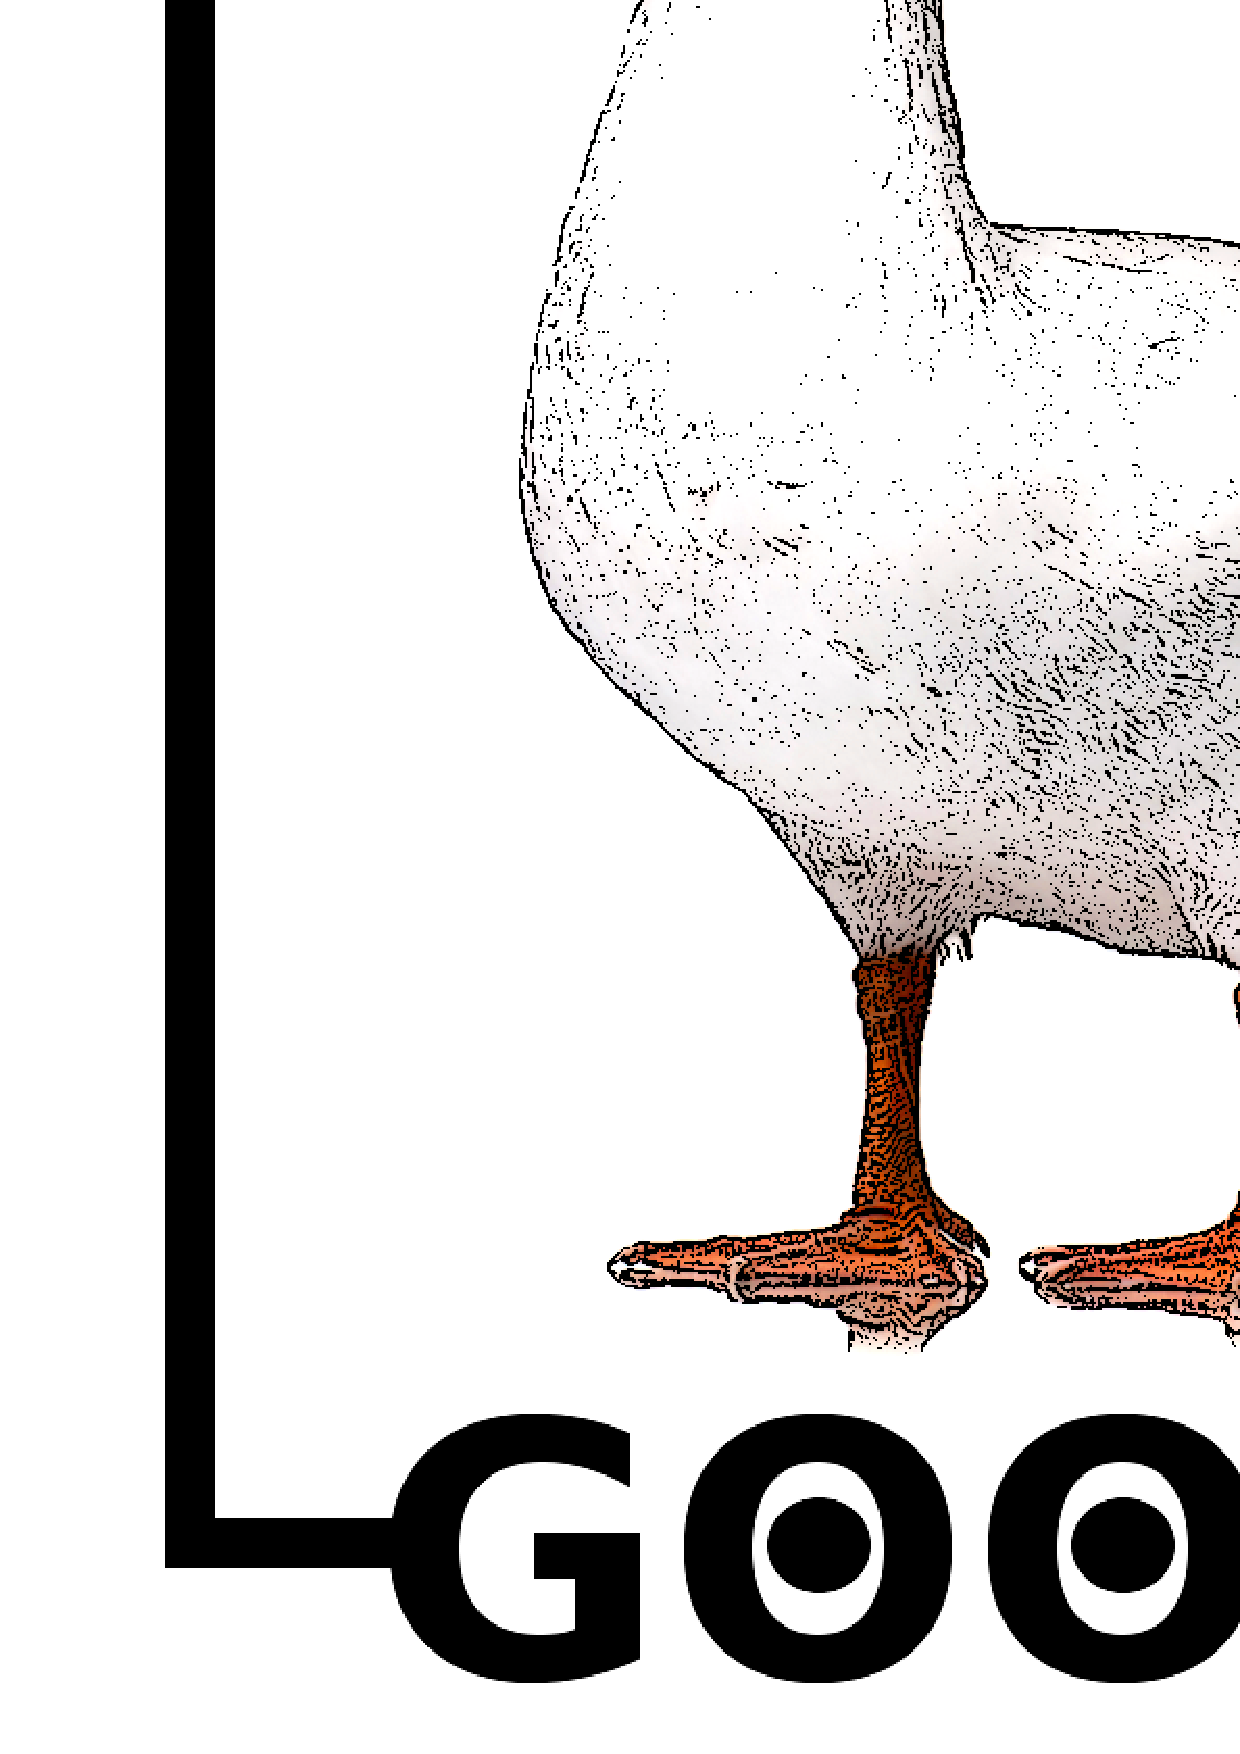
\includegraphics[width=5cm]{../imgs/logo.pdf}}
\label{logo}
\end{figure}
~\\
\textbf{A toolkit for DNA sequence\\ analysis and manipulation}
~\\~\\
\large
D. Pratas (pratas@ua.pt)\\
A. J. Pinho (ap@ua.pt)
~\\~\\
\small
IEETA/DETI, University of Aveiro, Portugal\\
~\\
Version 1.7.17
}
\date{}
\maketitle

\tableofcontents

%%%%%%%%%%%%%%%%%%%%%%%%%%%%%%%%%%%%%%%%%%%%%%%%%%%%%%%%%%%%%%%%%%%%%%%%%%%%%%%%
%%%%%%%%%%%%%%%%%%%%%%%%%%%%%%%%%%%%%%%%%%%%%%%%%%%%%%%%%%%%%%%%%%%%%%%%%%%%%%%%
%%%%%%%%%%%%%%%%%%%%%%%%%%%%%%%%%%%%%%%%%%%%%%%%%%%%%%%%%%%%%%%%%%%%%%%%%%%%%%%%
\chapter*{1. Introduction}
\addcontentsline{toc}{chapter}{1. Introduction}
\label{intro}

Recent advances in {DNA} sequencing have revolutionized the field of genomics,
making it possible for research groups to generate large amounts of sequenced
data, very rapidly and at substantially lower cost. Its storage have been
made using specific file formats, such as FASTQ and FASTA. Therefore, its
analysis and manipulation is crucial \cite{Buermans-2014a}. Several
frameworks for analysis and manipulation emerged, namely \texttt{GALAXY}
\cite{Giardine-2005a}, \texttt{GATK} \cite{DePristo-2011a}, \texttt{HTSeq}
\cite{Anders-2014a}, \texttt{MEGA} \cite{Kumar-2016a}, among others.
In the majority, these frameworks require licenses and do not provide
a low level access to the information, since they are commonly approached
by scripting or interfaces.

We describe \texttt{GOOSE}, a (free) novel toolkit for analyzing and manipulating
FASTA-FASTQ formats and sequences (DNA, amino acids, text), with many 
complementary tools. The toolkit is for Linux-based systems, built for fast 
processing. \texttt{GOOSE} supports pipes for easy integration. It includes tools 
for information display, randomizing, edition, conversion, extraction, 
searching, calculation and visualization. \texttt{GOOSE} is prepared to deal with
very large datasets, typically in the scale Gigabytes or Terabytes. 

The toolkit is a command line version, using the prefix ``goose-'' 
followed by the suffix with the respective name of the program.
\texttt{GOOSE} is implemented in \texttt{C} language and it is available, 
under GPLv3, at:
\begin{lstlisting}
https://pratas.github.io/goose
\end{lstlisting}

\section*{1.1 Installation}
\addcontentsline{toc}{section}{1.1~~~Installation}

For \texttt{GOOSE} installation, run:
\begin{lstlisting}
git clone https://github.com/pratas/goose.git
cd goose/src/
make
\end{lstlisting}

\section*{1.2 License}
\addcontentsline{toc}{section}{1.2~~~License}

The license is \textbf{GPLv3}. In resume, everyone is permitted to copy and 
distribute verbatim copies of this license document, but changing it is not 
allowed. For details on the license, consult: \url{http://www.gnu.org/licenses/gpl-3.0.html}.

%%%%%%%%%%%%%%%%%%%%%%%%%%%%%%%%%%%%%%%%%%%%%%%%%%%%%%%%%%%%%%%%%%%%%%%%%%%%%%%%
%%%%%%%%%%%%%%%%%%%%%%%%%%%%%%%%%%%%%%%%%%%%%%%%%%%%%%%%%%%%%%%%%%%%%%%%%%%%%%%%
%%%%%%%%%%%%%%%%%%%%%%%%%%%%%%%%%%%%%%%%%%%%%%%%%%%%%%%%%%%%%%%%%%%%%%%%%%%%%%%%
\chapter*{2. FASTQ tools}
\addcontentsline{toc}{chapter}{2. FASTQ tools}
\label{fastq}

Current available tools for FASTQ format analysis and manipulation include:
\begin{enumerate}

\item \texttt{goose-fastq2fasta}
\item \texttt{goose-fastq2mfasta}
\item \texttt{goose-fastqclustreads}
\item \texttt{goose-FastqExcludeN}
\item \texttt{goose-FastqExtractQualityScores}
\item \texttt{goose-FastqInfo}
\item \texttt{goose-FastqMaximumReadSize}
\item \texttt{goose-FastqMinimumLocalQualityScoreForward}
\item \texttt{goose-FastqMinimumLocalQualityScoreReverse}
\item \texttt{goose-FastqMinimumQualityScore}
\item \texttt{goose-FastqMinimumReadSize}

\item \texttt{goose-count}
\item \texttt{goose-extractreadbypattern}



\item \texttt{goose-fastqpack}
\item \texttt{goose-fastqsimulation}
\item \texttt{goose-FastqSplit}
\item \texttt{goose-FastqTrimm}
\item \texttt{goose-fastqunpack}
\item \texttt{goose-filter}
\item \texttt{goose-findnpos}

\item \texttt{goose-genrandomdna}
\item \texttt{goose-getunique}
\item \texttt{goose-info}
\item \texttt{goose-mfmotifcoords}



\item \texttt{goose-mutatefastq}
\item \texttt{goose-newlineonnewx}
\item \texttt{goose-period}
\item \texttt{goose-permuteseqbyblocks}


\item \texttt{goose-randfastqextrachars}

\item \texttt{goose-real2binthreshold}
\item \texttt{goose-reducematrixbythreshold}
\item \texttt{goose-renamehumanheaders}


\item \texttt{goose-searchphash}

\item \texttt{goose-seq2fasta}
\item \texttt{goose-seq2fastq}
\item \texttt{goose-SequenceToGroupSequence}
\item \texttt{goose-splitreads}

\item \texttt{goose-wsearch}
\end{enumerate}

%%%%%%%%%%%%%%%%%%%%%%%%%%%%%%%%%%%%%%%%%%%%%%%%%%%%%%%%%%%%%%%%%%%%%%%%%%%%%%%%
%%%%%%%%%%%%%%%%%%%%%%%%%%%%%%%%%%%%%%%%%%%%%%%%%%%%%%%%%%%%%%%%%%%%%%%%%%%%%%%%
%%%%%%%%%%%%%%%%%%%%%%%%%%%%%%%%%%%%%%%%%%%%%%%%%%%%%%%%%%%%%%%%%%%%%%%%%%%%%%%%
\chapter*{3. FASTA tools}
\addcontentsline{toc}{chapter}{3. FASTA tools}
\label{fasta}

\begin{enumerate}
\item \texttt{goose-fasta2seq}
\item \texttt{goose-fastaextract}
\item \texttt{goose-fastainfo}
\item \texttt{goose-mutatefasta}
\item \texttt{goose-randfastaextrachars}
\item \texttt{goose-geco}
\item \texttt{goose-gede}
\item \texttt{goose-mutatedna}
\item \texttt{goose-randseqextrachars}
\item \texttt{goose-reverse}: it reverses the order of a sequence.
\item \texttt{goose-reverselm}: it reverses the order of a large sequence. Low memory usage for large files.
\end{enumerate}

%%%%%%%%%%%%%%%%%%%%%%%%%%%%%%%%%%%%%%%%%%%%%%%%%%%%%%%%%%%%%%%%%%%%%%%%%%%%%%%%
%%%%%%%%%%%%%%%%%%%%%%%%%%%%%%%%%%%%%%%%%%%%%%%%%%%%%%%%%%%%%%%%%%%%%%%%%%%%%%%%
%%%%%%%%%%%%%%%%%%%%%%%%%%%%%%%%%%%%%%%%%%%%%%%%%%%%%%%%%%%%%%%%%%%%%%%%%%%%%%%%
\chapter*{4. Amino acid sequence tools}
\addcontentsline{toc}{chapter}{4. Sequence tools}
\label{seq}

Current available amino acid sequence tools, for analysis and manipulation, are:
\begin{enumerate}
\item \texttt{goose-AminoAcidToGroup}
\item \texttt{goose-ProteinToPseudoDNA}
\end{enumerate}

\section*{4.1 Program goose-AminoAcidToGroup}
\addcontentsline{toc}{section}{4.1~~~Program goose-AminoAcidToGroup}

The \texttt{goose-AminoAcidToGroup} converts an amino acid sequence to a group 
sequence.\\
For help type:
\begin{lstlisting}
./goose-AminoAcidToGroup -h
\end{lstlisting}
In the following subsections, we explain the input and output paramters.

\subsection*{Input parameters}
\addcontentsline{toc}{subsection}{4.1.1~~~Input parameters}

The \texttt{goose-AminoAcidToGroup} program needs two streams for the computation,
namely the input and output standard. The input stream is an amino acid sequence.
The attribution is given according to:
\begin{lstlisting}
Usage: ./goose-AminoAcidToGroup < in.prot > out.group
It converts a amino acid sequence to a group sequence.
Table:
Prot	Group
R	P
H	P  Amino acids with electric charged side chains: POSITIVE
K	P
-	-
D	N
E	N  Amino acids with electric charged side chains: NEGATIVE
-	-
S	U
T	U
N	U  Amino acids with electric UNCHARGED side chains
Q	U
-	-
C	S
U	S
G	S  Special cases
P	S
-	-
A	H
V	H
I	H
L	H
M	H  Amino acids with hydrophobic side chains
F	H
Y	H
W	H
-	-
*	*  Others
X	X  Unknown
\end{lstlisting}
It can be used to group amino acids by properties, such as electric charge (positive
and negative), uncharged side chains, hydrophobic side chains and special cases.
An example on such an input file is:
\begin{lstlisting}
IPFLLKKQFALADKLVLSKLRQLLGGRIKMMPCGGAKLEPAIGLFFHAIGINIKLGYGMTETTATVSCWHDFQFNPNSIG
TLMPKAEVKIGENNEILVRGGMVMKGYYKKPEETAQAFTEDGFLKTGDAGEFDEQGNLFITDRIKELMKTSNGKYIAPQY
IESKIGKDKFIEQIAIIADAKKYVSALIVPCFDSLEEYAKQLNIKYHDRLELLKNSDILKMFE
\end{lstlisting}

\subsection*{Output}
\addcontentsline{toc}{subsection}{4.1.2~~~Output}

The output of the \texttt{goose-AminoAcidToGroup} program is a group sequence.\\
An example, for the input, is:
\begin{lstlisting}
HSHHHPPUHHHHNPHHHUPHPUHHSSPHPHHSSSSHPHNSHHSHHHPHHSHUHPHSHSHUNUUHUHUSHPNHUHUSUUHS
UHHSPHNHPHSNUUNHHHPSSHHHPSHHPPSNNUHUHHUNNSHHPUSNHSNHNNUSUHHHUNPHPNHHPUUUSPHHHSUH
HNUPHSPNPHHNUHHHHHNHPPHHUHHHHSSHNUHNNHHPUHUHPHPNPHNHHPUUNHHPHHN
\end{lstlisting}

\section*{4.2 Program goose-ProteinToPseudoDNA}
\addcontentsline{toc}{section}{4.2~~~Program goose-ProteinToPseudoDNA}

The \texttt{goose-ProteinToPseudoDNA} converts an amino acid (protein) sequence to a pseudo DNA sequence.\\
For help type:
\begin{lstlisting}
./goose-ProteinToPseudoDNA -h
\end{lstlisting}
In the following subsections, we explain the input and output paramters.

\subsection*{Input parameters}
\addcontentsline{toc}{subsection}{4.2.1~~~Input parameters}

The \texttt{goose-ProteinToPseudoDNA} program needs two streams for the computation,
namely the input and output standard. The input stream is an amino acid sequence.
The attribution is given according to:
\begin{lstlisting}
Usage: ./goose-ProteinToPseudoDNA < in.prot > out.dna
It converts a protein sequence to a pseudo DNA sequence.
Table:
Prot  DNA
A	  GCA
C	  TGC
D	  GAC
E	  GAG
F	  TTT
G	  GGC
H	  CAT
I	  ATC
K	  AAA
L	  CTG
M	  ATG
N	  AAC
P	  CCG
Q	  CAG
R	  CGT
S     TCT
T	  ACG
V	  GTA
W	  TGG
Y	  TAC
*	  TAG
X	  GGG
\end{lstlisting}
It can be used to generate pseudo-DNA with characteristics passed by amino acid (protein) sequences. An example on such an input file is:
\begin{lstlisting}
IPFLLKKQFALADKLVLSKLRQLLGGRIKMMPCGGAKLEPAIGLFFHAIGINIKLGYGMTETTATVSCWHDFQFNPNSIG
TLMPKAEVKIGENNEILVRGGMVMKGYYKKPEETAQAFTEDGFLKTGDAGEFDEQGNLFITDRIKELMKTSNGKYIAPQY
IESKIGKDKFIEQIAIIADAKKYVSALIVPCFDSLEEYAKQLNIKYHDRLELLKNSDILKMFE
\end{lstlisting}

\subsection*{Output}
\addcontentsline{toc}{subsection}{4.2.2~~~Output}

The output of the \texttt{goose-ProteinToPseudoDNA} program is a DNA sequence.\\
An example, for the input, is:
\begin{lstlisting}
ATCCCGTTTCTGCTGAAAAAACAGTTTGCACTGGCAGACAAACTGGTACTGTCTAAACTGCGTCAGCTGCTGGGCGGCCG
TATCAAAATGATGCCGTGCGGCGGCGCAAAACTGGAGCCGGCAATCGGCCTGTTTTTTCATGCAATCGGCATCAACATCA
AACTGGGCTACGGCATGACGGAGACGACGGCAACGGTATCTTGCTGGCATGACTTTCAGTTTAACCCGAACTCTATCGGC
ACGCTGATGCCGAAAGCAGAGGTAAAAATCGGCGAGAACAACGAGATCCTGGTACGTGGCGGCATGGTAATGAAAGGCTA
CTACAAAAAACCGGAGGAGACGGCACAGGCATTTACGGAGGACGGCTTTCTGAAAACGGGCGACGCAGGCGAGTTTGACG
AGCAGGGCAACCTGTTTATCACGGACCGTATCAAAGAGCTGATGAAAACGTCTAACGGCAAATACATCGCACCGCAGTAC
ATCGAGTCTAAAATCGGCAAAGACAAATTTATCGAGCAGATCGCAATCATCGCAGACGCAAAAAAATACGTATCTGCACT
GATCGTACCGTGCTTTGACTCTCTGGAGGAGTACGCAAAACAGCTGAACATCAAATACCATGACCGTCTGGAGCTGCTGA
AAAACTCTGACATCCTGAAAATGTTTGAG
\end{lstlisting}



%%%%%%%%%%%%%%%%%%%%%%%%%%%%%%%%%%%%%%%%%%%%%%%%%%%%%%%%%%%%%%%%%%%%%%%%%%%%%%%%
%%%%%%%%%%%%%%%%%%%%%%%%%%%%%%%%%%%%%%%%%%%%%%%%%%%%%%%%%%%%%%%%%%%%%%%%%%%%%%%%
%%%%%%%%%%%%%%%%%%%%%%%%%%%%%%%%%%%%%%%%%%%%%%%%%%%%%%%%%%%%%%%%%%%%%%%%%%%%%%%%
\chapter*{5. General purpose tools}
\addcontentsline{toc}{chapter}{5. General purpose tools}
\label{seq}

\begin{enumerate}
\item \texttt{goose-comparativemap}: visualisation of comparative maps. It builds a image given specific patterns between two sequences.
\item \texttt{goose-BruteForceString}: it generates, line by line, multiple combinations of strings up to a certain size.
\item \texttt{goose-char2line}: it transforms each char into a char in each line.
\item \texttt{goose-sum}: it adds the second column value to the first column value.
\item \texttt{goose-min}: it finds the minimum value between two column values.
\item \texttt{goose-minus}: it substracts the second column value to the first column value.
\item \texttt{goose-max}: it finds the mmaximum value between two column values.
\item \texttt{goose-extract}: it extracts a subsequence of a sequence by coordinates.
\item \texttt{goose-segment}: it segments a sequence given a certain threshold.
\end{enumerate}





\addcontentsline{toc}{chapter}{Bibliography}
\bibliographystyle{IEEEtran}
\bibliography{defs,SPLc,SPLj,Cod,Bio,Book,Anc,Patho}

\end{document}
